\documentclass[12pt]{article}
\usepackage[margin=1.2in, top=0.5in]{geometry}
\usepackage[all]{nowidow}
\usepackage[hyperfigures=true, hidelinks, pdfhighlight=/N]{hyperref}
\usepackage[group-digits=false]{siunitx}
\usepackage{graphicx,amsmath,physics,tabto,float,amssymb,pgfplots,verbatim,tcolorbox}
\usepackage{listings,xcolor,subfig,caption,import,wrapfig}
\usepackage[numbered,framed]{matlab-prettifier}
\usepackage[version=4]{mhchem}
\numberwithin{equation}{section}
\numberwithin{figure}{section}
\numberwithin{table}{section}
\definecolor{stringcolor}{HTML}{C792EA}
\definecolor{codeblue}{HTML}{2162DB}
\definecolor{commentcolor}{HTML}{4A6E46}
\lstset{style=Matlab-editor}
\renewcommand{\lstlistingname}{Appendix}
\pgfplotsset{compat=1.17}

\begin{document}

\begin{center}
    {\huge Head-on Collisions of Nonlinear Schr\"odinger waves}\\
    \vspace{0.2in}
    \textbf{KDSMIL001 | June 2021}

    \section*{Abstract}\label{sec:Abstract}
    We will study the collisions of two solitons in media with saturation nonlinearity properties, as described by a nonlinear Schr\"odinger equation. This will be done using two different numerical methods, split step and implicit finite difference/Crank-Nicolson, in order to compare their benefits and drawbacks.
\end{center}

\section{Introduction}\label{sec:Introduction}
\par The equation we will investigate is 
\begin{equation}
    i\psi_t+\psi_{xx}+\frac{2|\psi|^2\psi}{1+S\sin|\psi|^2}
    \label{eqn:Main}
\end{equation}
with periodic boundary conditions and the initial conditions being two solitons separated by a sufficiently large distance ($\sim40$ units) given by
\begin{equation}
    \psi(x,0)=\sum_{j=1,2}A_j\sech[A_j(x-x_j)]e^{iv_j(x-x_j)}
    \label{eqn:IC}
\end{equation}
\par We will investigate this equation for different values of the saturation of nonlinearity $S$, velocities $v_j$, and initial separations $|x_2-x_1|$. We choose $A_j$ to be the same for all runs.
\par The two methods we plan to use work in very different ways. The implicit finite difference method, in this case it's specifically a Crank-Nicolson method, is conceptually much simpler. All that we do is approximate the derivative of our function using finite difference methods and solve a matrix equation at each time step to find the value of the function at the next time step. This is conceptually simple, but when it comes to actually doing the computation, because our step in both space in time need to be small in order for our finite difference approximations to be accurate, that means inverting an incredibly large matrix, which is simple but takes a lot of time.
\par In contrast to that, the split step method is conceptually quite challenging, requiring many complicated steps to arrive at a way to solve for the next time step. This method of solving for the next time step, however, is computationally very simple; all it requires is doing the Fourier Fast Transform and Inverse Fourier Fast Transform and we have our solution. This means that, in theory, the split step method is much less computationally expensive. 

\section{Method}\label{sec:Method}
\par Our implementation of the split step method is fairly simple, below are the vital lines.
\begin{lstlisting}
n=[0:N/2-1 -N/2:-1].^2;
n=exp(-1i*tau*4*pi^2/L^2*n);

psi=psi.*exp((1i*tau*2*abs(psi).^2)...
    ./(1+S.*sin(abs(psi).^2)));
psi=ifft(n.*fft(psi));
\end{lstlisting}
The first 2 lines are done before we iterate and we do the last 3 for each time step, saving the solution to an array to be plotted at the end. Note the only computationally expensive things being done are the Fourier Fast Transforms, which are done very easily and quickly.
\par The finite difference implementation is slightly longer but also quite simple.
\begin{lstlisting}
A=diag(s/2*ones(N-1,1),1)+diag((1i-s)*ones(N,1),0)...
    +diag(s/2*ones(N-1,1),-1);
A(1,N)=s/2;
A(N,1)=s/2;
B=inv(A);

rhs(2:N-1)=-s/2*psi(1:N-2)+(1i+s)*psi(2:N-1)-...
    (2*tau*abs(psi(2:N-1)).^2)./(1+S*sin...
    (abs(psi(2:N-1)).^2)).*psi(2:N-1)-s/2*psi(3:N);
rhs(1)=-s/2*psi(N)+(1i+s)*psi(1)-(2*tau*abs(psi(1)).^2)...
    /(1+S*sin(abs(psi(1)).^2)).*psi(1)-s/2*psi(2);
rhs(N)=-s/2*psi(N-1)+(1i+s)*psi(N)-(2*tau*abs(psi(N)).^2)...
    /(1+S*sin(abs(psi(N)).^2)).*psi(N)-s/2*psi(1);
psi = B*rhs;
\end{lstlisting}
where $s=\tau/h^2$ and from line 6 we iterate through the time steps. The computationally expensive thing here is the multiplication of the matrix \texttt{B}. Normally this isn't a very hard thing to do but since we have on the order of 1000 spatial mesh points, it just takes a long time since matrix is then on the order of $1000\times1000$.\newline

\par The parameters that we could change to optimize each method were as follows: $L$ is the length of the spatial interval, remained at 100 for all tests we made. $N$ is the number of spatial mesh points, which was varied between methods. \texttt{tMax} is the number of time steps taken in a run, which varied depending on velocities and spacing in order for the resulting plots to look nicer. $h=L/N$ is the spatial step and $\tau=h^2/3$ is the time step. 
\par In order to compare the two methods on fair grounds we calibrated each so that the conserved quantity $N$, given by
\begin{equation}
    I=\int_{-\infty}^{+\infty}\lvert\psi\rvert^2dx
\end{equation}
for one soliton for a small amount of time, stays within some chosen accuracy $\varepsilon$. We chose $\varepsilon=\num{1e-5}$ and for split step there was no problem staying within that accuracy as well as keeping the runtime to a reasonable amount. In fact it conserved the quantity to an accuracy of around $\num{1e-12}$ consistently. For the finite difference method, it was a little bit more complicated. We could just about get the accuracy desired with $N=2000$. Increasing $N$ does improve the accuracy but it means the runtime goes to ridiculous amounts, which will be discussed later on.
\par To compare the two methods we simulated a number of collisions varying $S$, $v_j$, and $|x_2-x_1|$ as stated before. The plots of the time evolutions of each variation are in \autoref{sec:Results}.

\section{Results}\label{sec:Results}
Let us begin by comparing the two methods on a baseline. Going forward, unless specifically stated, these will be the parameters used: $A_1=A_2=1$, $x_1=-x_2=-20$, $v_1=-v_2=5$, $S=0.5$, $h=L/N$, $\tau=h^2/3$.

\begin{figure}[H]%
    \centering
    \subfloat[\centering Split Step]{\scalebox{0.5}{\includegraphics{Plots/splitStep_Main.eps}}}
    \,
    \subfloat[\centering Implicit finite difference]{\scalebox{0.5}{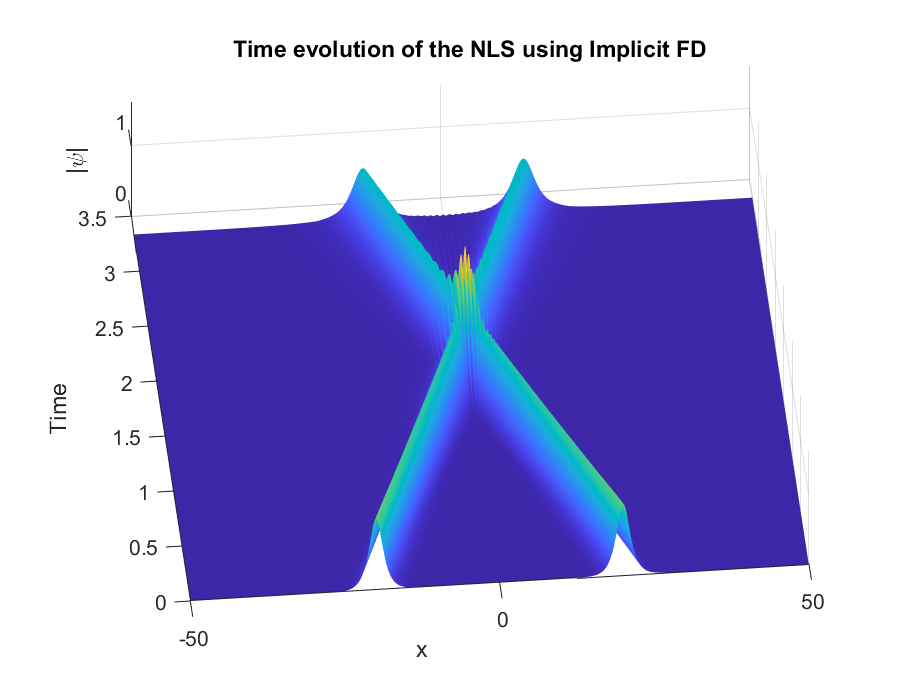
\includegraphics{Plots/FD_Main.eps}}}
    \caption{Time evolution of the colliding waves using the baseline parameters.}
    \label{fig:Mains}
\end{figure}
\par As an aside, there will be discrepancies in the final time on the Time axis for all of these comparisons. This is a result of the differences in $\tau$ and $h$ to keep the accuracy in check.

\begin{figure}[H]%
    \centering
    \subfloat[\centering Split Step]{\scalebox{0.5}{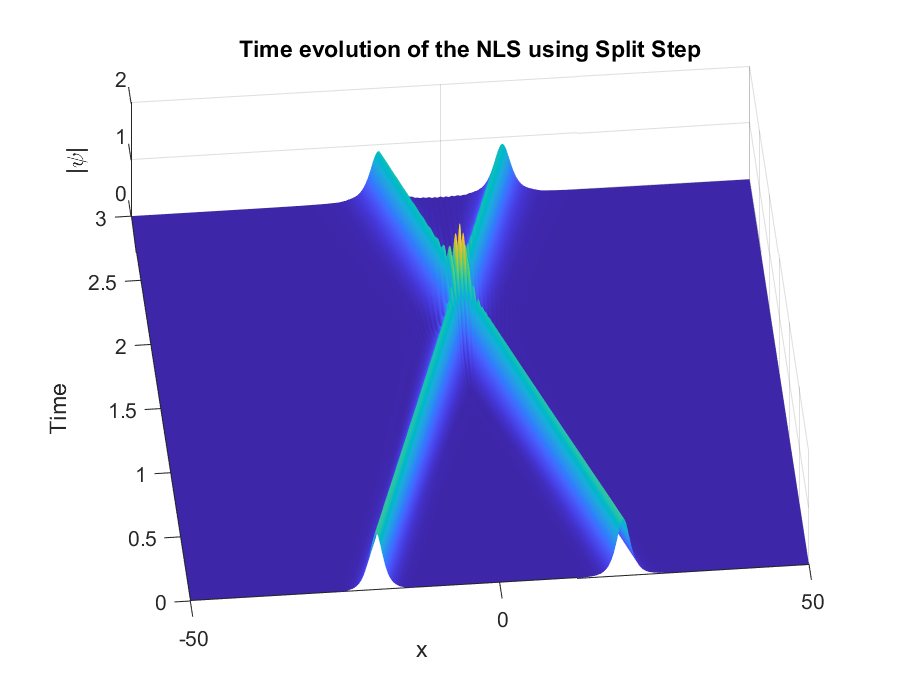
\includegraphics{Plots/splitStep_S02.eps}}}
    \,
    \subfloat[\centering Implicit finite difference]{\scalebox{0.5}{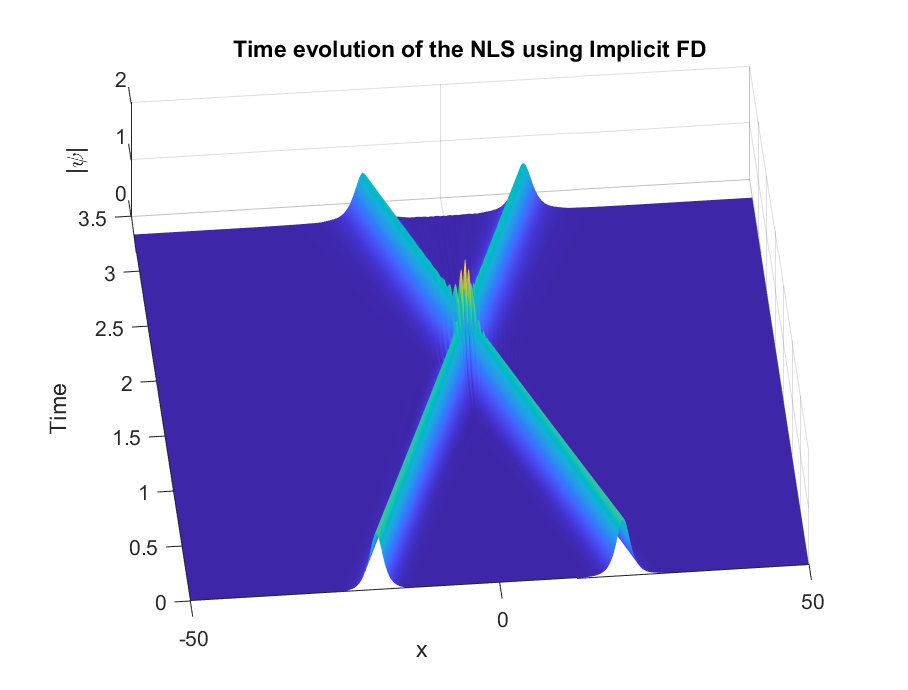
\includegraphics{Plots/FD_S02.eps}}}
    \caption{Time evolution of the colliding waves with $S=0.2$.}
    \label{fig:S02}
\end{figure}

\begin{figure}[H]%
    \centering
    \subfloat[\centering Split Step]{\scalebox{0.5}{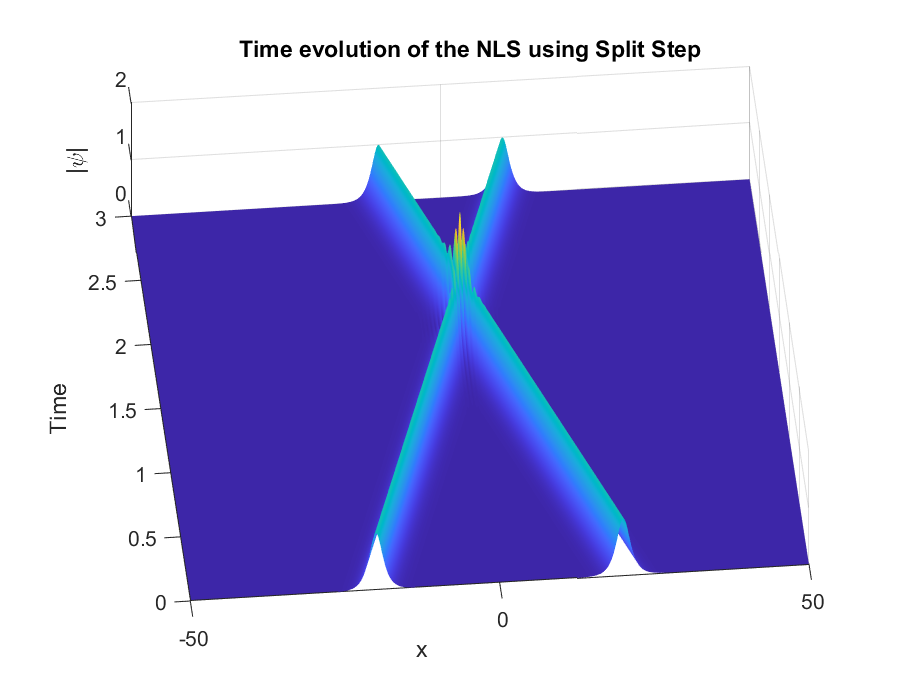
\includegraphics{Plots/splitStep_S0.eps}}}
    \,
    \subfloat[\centering Implicit finite difference]{\scalebox{0.5}{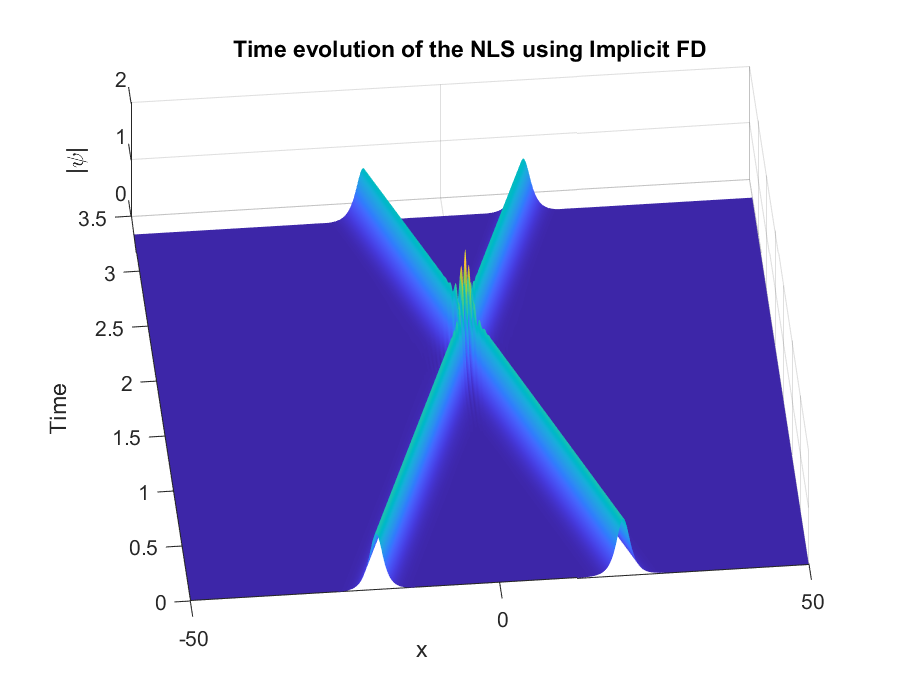
\includegraphics{Plots/FD_S0.eps}}}
    \caption{Time evolution of the colliding waves with $S=0$.}
    \label{fig:S0}
\end{figure}

\begin{figure}[H]%
    \centering
    \subfloat[\centering Split Step]{\scalebox{0.5}{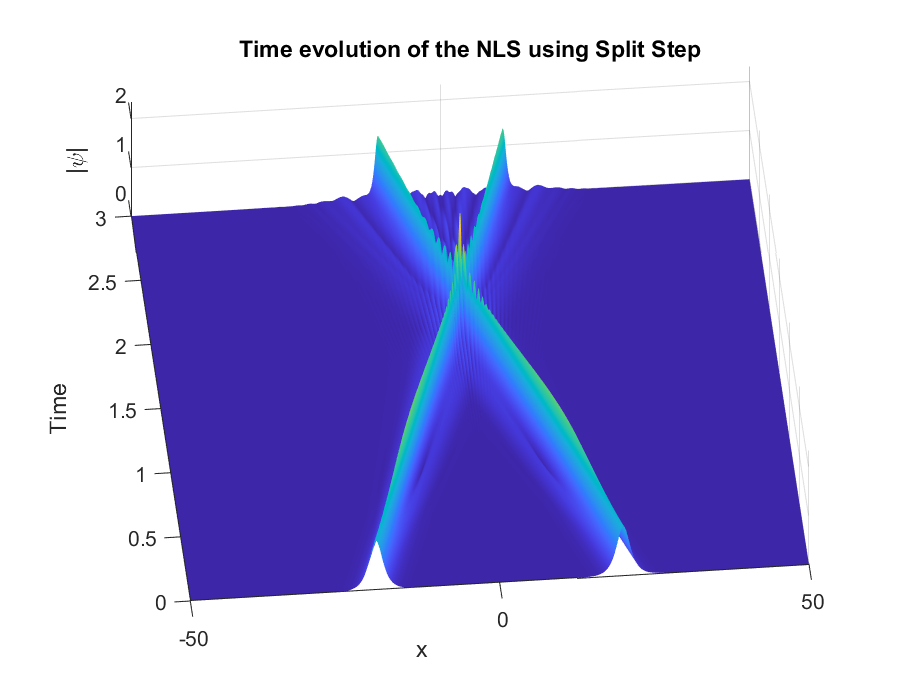
\includegraphics{Plots/splitStep_S-05.eps}}}
    \,
    \subfloat[\centering Implicit finite difference]{\scalebox{0.5}{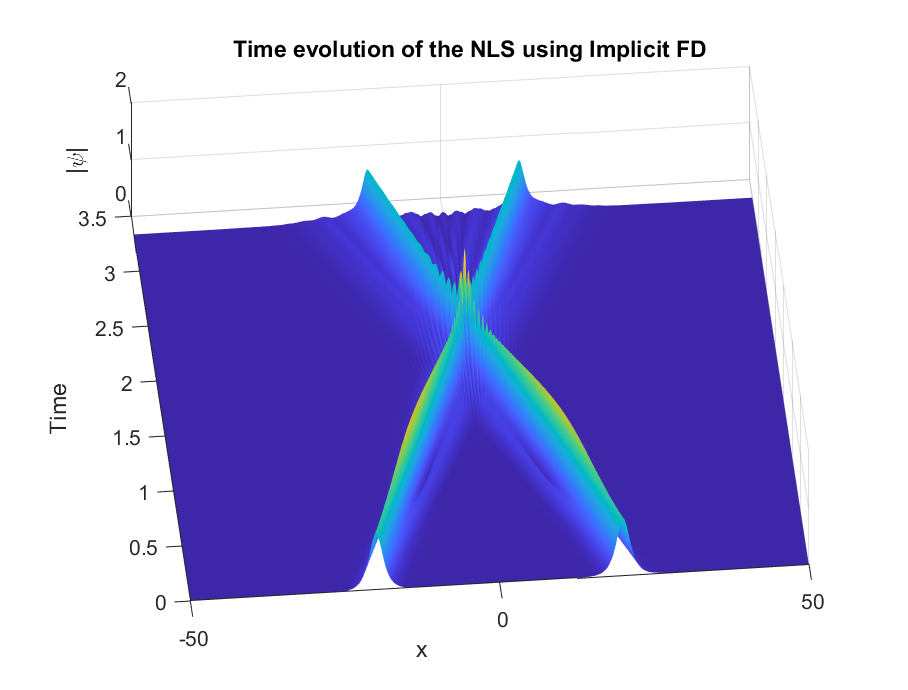
\includegraphics{Plots/FD_S-05.eps}}}
    \caption{Time evolution of the colliding waves with $S=-0.5$.}
    \label{fig:S-05}
\end{figure}

\begin{figure}[H]%
    \centering
    \subfloat[\centering Split Step]{\scalebox{0.5}{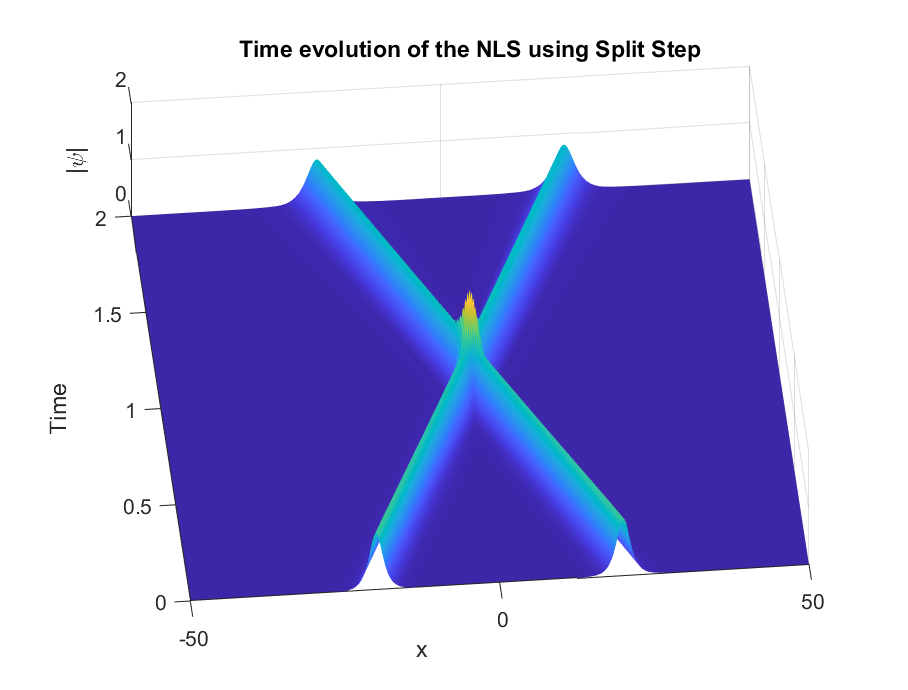
\includegraphics{Plots/splitStep_v10.eps}}}
    \,
    \subfloat[\centering Implicit finite difference]{\scalebox{0.5}{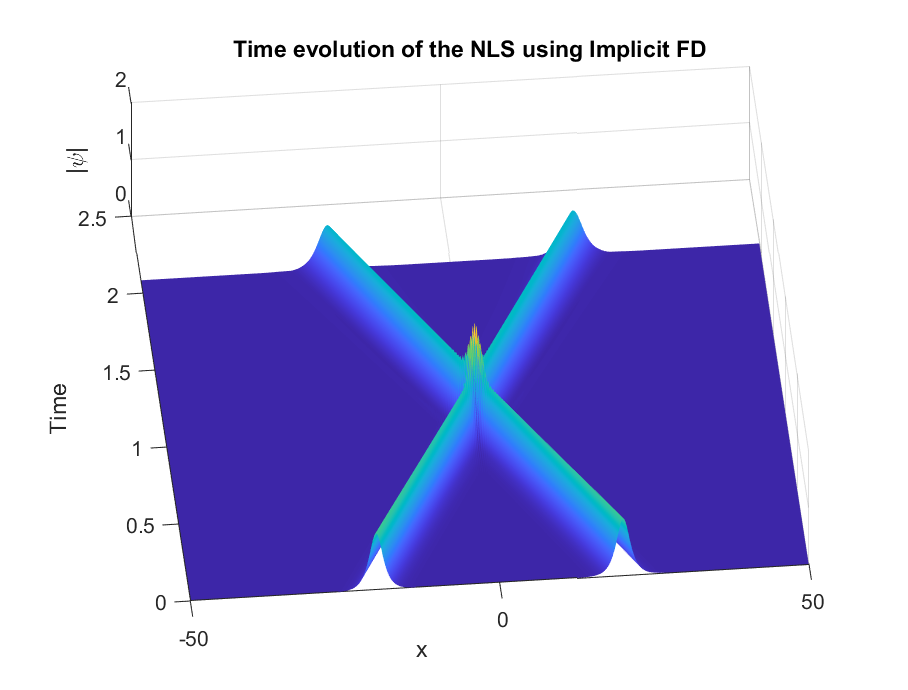
\includegraphics{Plots/FD_v10.eps}}}
    \caption{Time evolution of the colliding waves with $|v|=10$.}
    \label{fig:v10}
\end{figure}

\begin{figure}[H]%
    \centering
    \subfloat[\centering Split Step]{\scalebox{0.5}{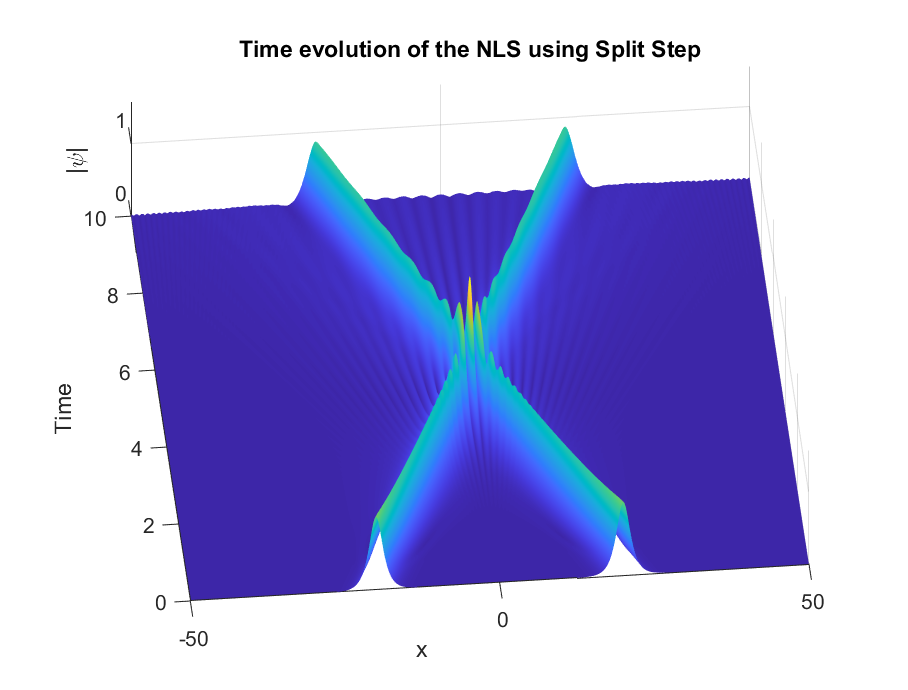
\includegraphics{Plots/splitStep_v2.eps}}}
    \,
    \subfloat[\centering Implicit finite difference]{\scalebox{0.5}{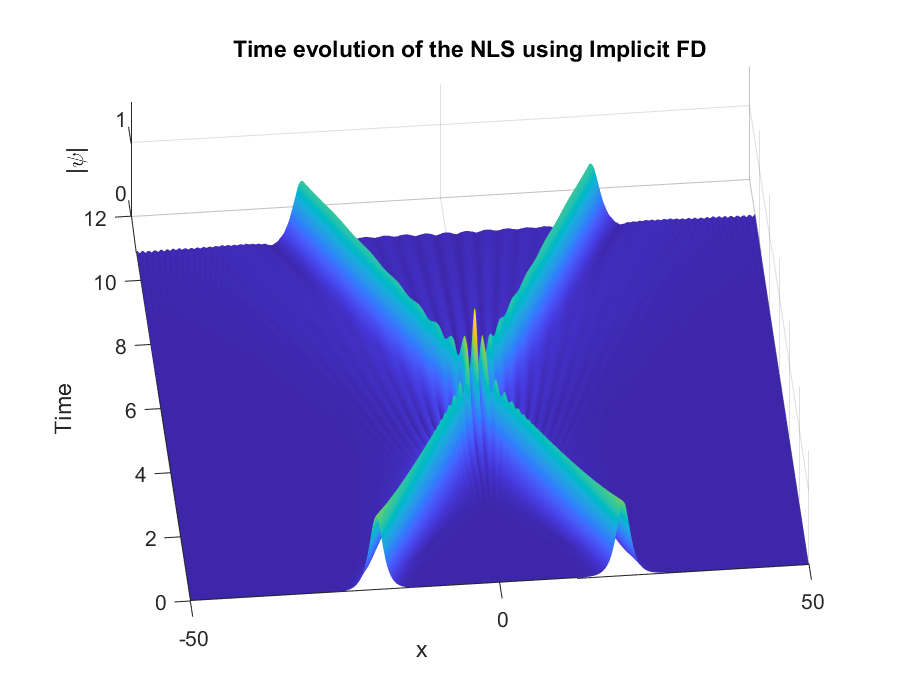
\includegraphics{Plots/FD_v2.eps}}}
    \caption{Time evolution of the colliding waves with $|v|=2$.}
    \label{fig:v2}
\end{figure}

\begin{figure}[H]%
    \centering
    \subfloat[\centering Split Step]{\scalebox{0.5}{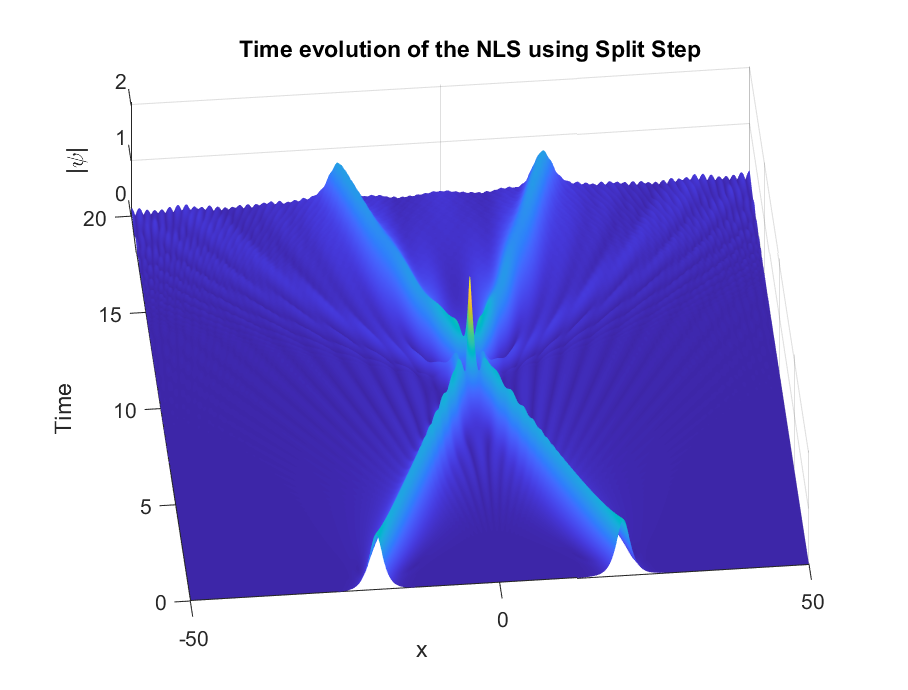
\includegraphics{Plots/splitStep_v1.eps}}}
    \,
    \subfloat[\centering Implicit finite difference]{\scalebox{0.5}{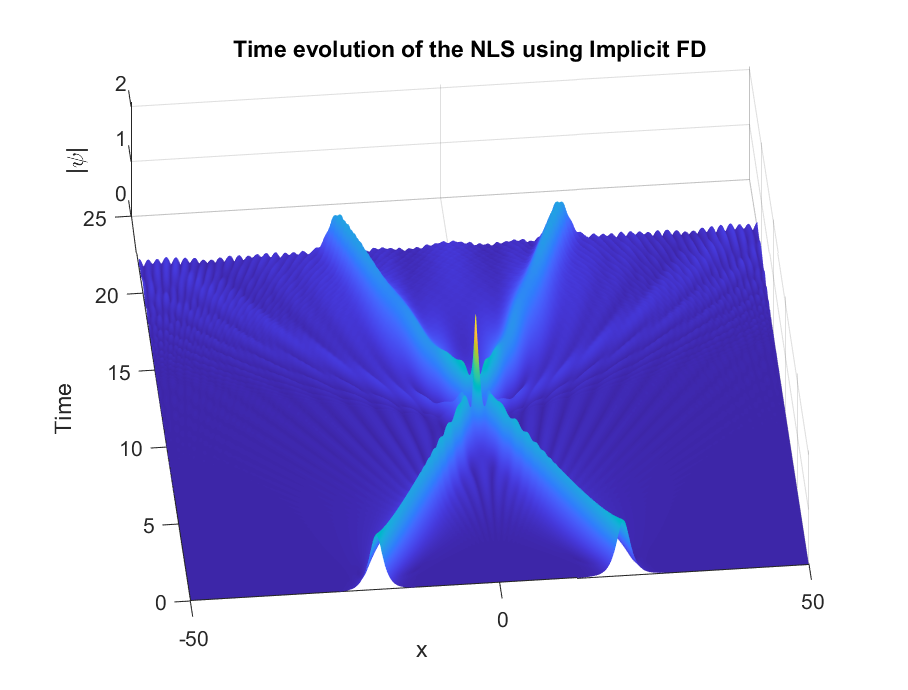
\includegraphics{Plots/FD_v1.eps}}}
    \caption{Time evolution of the colliding waves with $|v|=1$.}
    \label{fig:v1}
\end{figure}

\begin{figure}[H]%
    \centering
    \subfloat[\centering Split Step]{\scalebox{0.5}{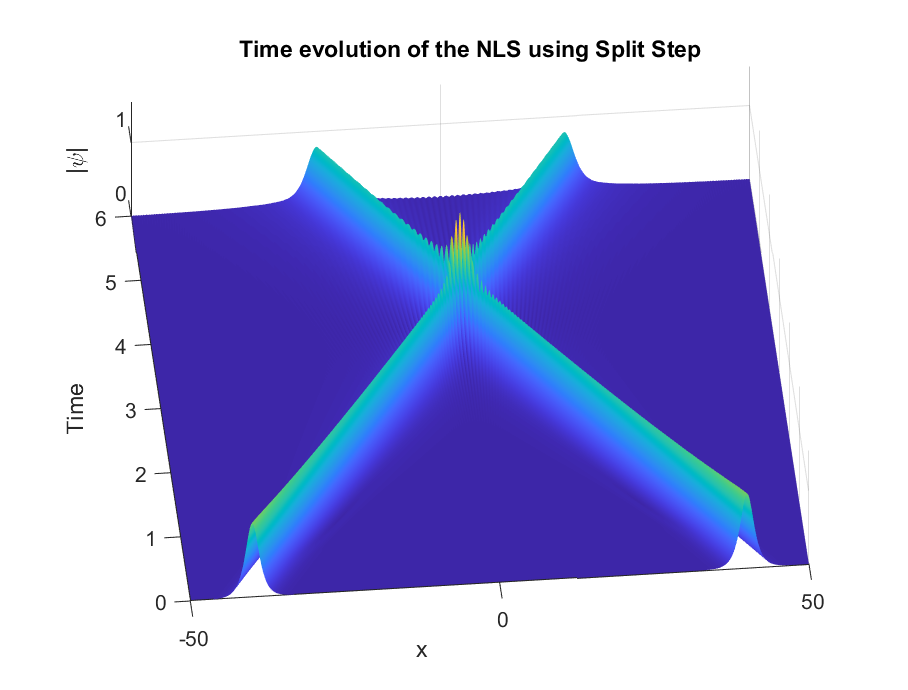
\includegraphics{Plots/splitStep_x80.eps}}}
    \,
    \subfloat[\centering Implicit finite difference]{\scalebox{0.5}{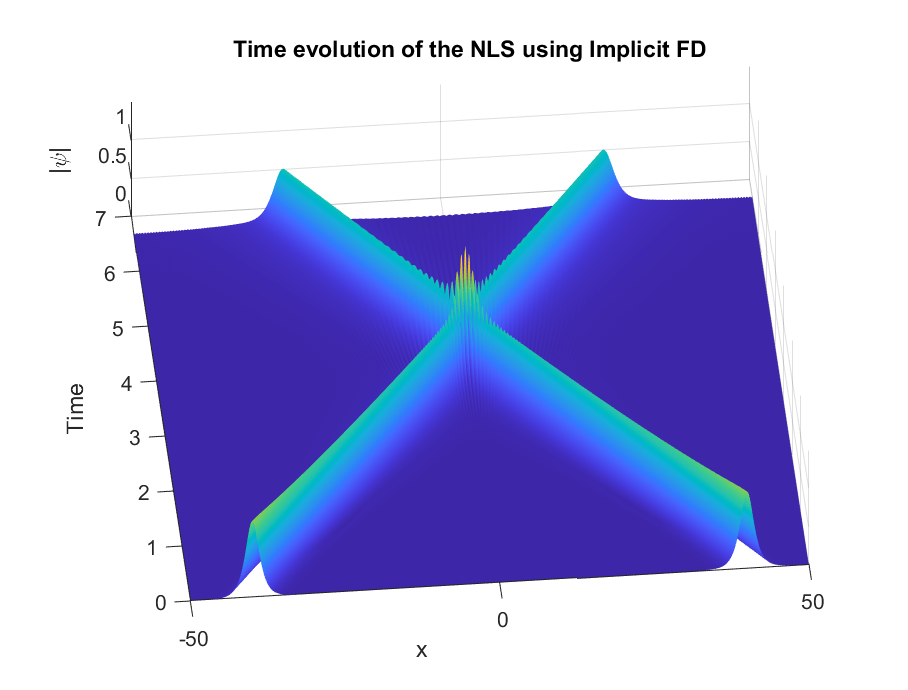
\includegraphics{Plots/FD_x80.eps}}}
    \caption{Time evolution of the colliding waves with $|x_2-x_1|=80$.}
    \label{fig:x80}
\end{figure}

\begin{figure}[H]%
    \centering
    \subfloat[\centering Split Step]{\scalebox{0.5}{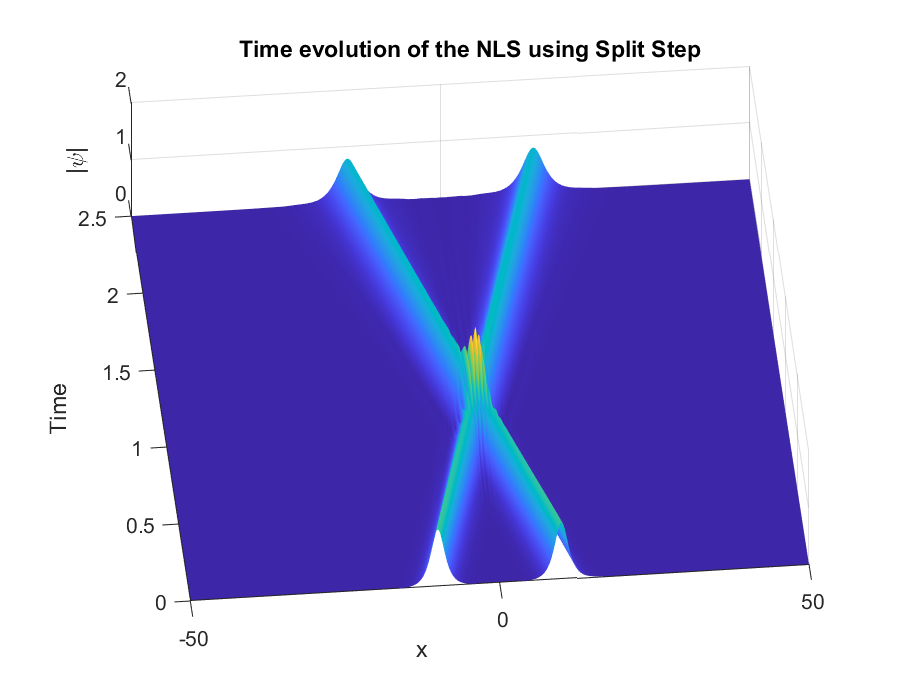
\includegraphics{Plots/splitStep_x20.eps}}}
    \,
    \subfloat[\centering Implicit finite difference]{\scalebox{0.5}{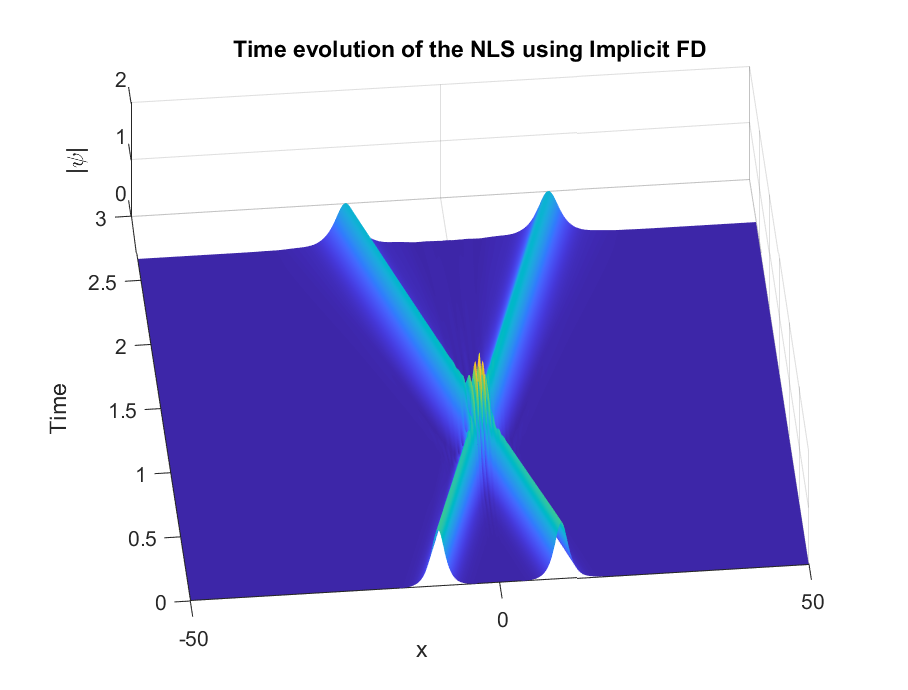
\includegraphics{Plots/FD_x20.eps}}}
    \caption{Time evolution of the colliding waves with $|x_2-x_1|=20$.}
    \label{fig:x20}
\end{figure}

\begin{figure}[H]%
    \centering
    \subfloat[\centering Split Step]{\scalebox{0.5}{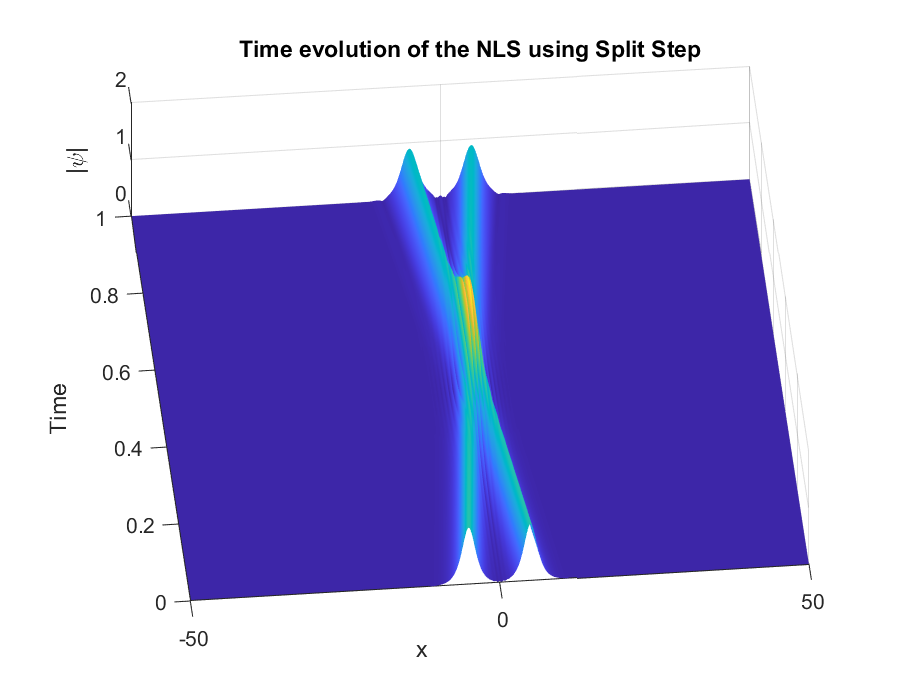
\includegraphics{Plots/splitStep_x10.eps}}}
    \,
    \subfloat[\centering Implicit finite difference]{\scalebox{0.5}{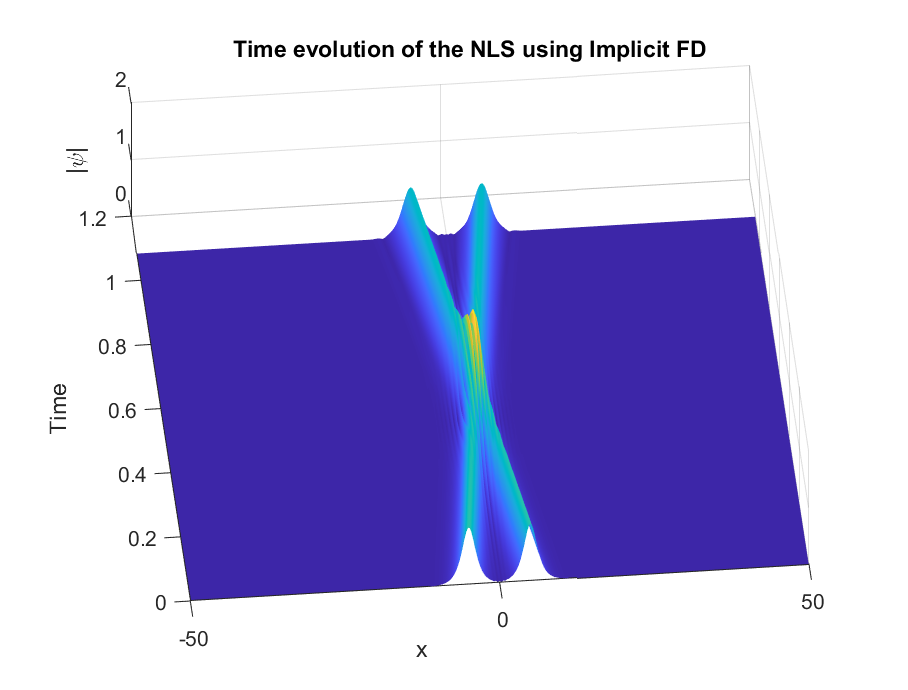
\includegraphics{Plots/FD_x10.eps}}}
    \caption{Time evolution of the colliding waves with $|x_2-x_1|=10$.}
    \label{fig:x10}
\end{figure}

\par Looking purely at the results, it's clear that the two methods produce similar solutions with similar behaviour, most notably the fact that as the two solitons collide we see oscillations that do not line up with how we expect solitons to interact as they shouldn't interact at all. Nevertheless if we examine the shape of the solution before and after collision we see that for all variations apart from $S=0$, we see that the solitons devolve into oscillations. This is most noticeable for $S=-0.5$ and $|v|=1$. From this we can say that if there is some non-zero saturation of nonlinearity the solitons do, in fact, interact and result in strange, undesirable behaviour.
\par Regarding the differences between values of $S$, we see that for negative $S$ the solution behaves quite strangely with growing amplitudes and noise around each soliton evolving over time. This is present for positive $S$ but it seems to be less so, and also seems to be less prevalent for values of $S$ closer to 0. Also note that the finite difference method seemed to consistently exaggerate deviations compared to split step. 
\par The differences when it came to $|v|$ are interesting. Thinking about it before we ran the simulations we expected that larger velocities would result in instability since the program is making larger jumps for each time step, but as it turns out we appear to see the opposite happen. For $|v|=10$ we see a very smooth solution, no oscillations beyond those seen when the solitons combine, but for smaller velocities, namely $|v|=1$ the solution seems to devolve entirely. This leads us to believe that both methods are stable when it comes to different velocities and this is a result of the saturation of nonlinearity, since these runs were done with $S=0.5$, and the lower velocities just amplified that noise. Again notice the finite difference method showing larger deviations. 
\par And finally the variations in starting distance for the solitons. This seemed to have little to no effect on the shape and behaviour of the solutions. The most notable thing is that for $|x_2-x_1|=80$ we see oscillations start to form between the solitons at the end of the run, but we suspect this is simply because the program had to run for longer in order for the solitons to collide and as time goes on those oscillations grow.
\newline
\par Lastly let us look at the main difference that we noticed between the two methods: The runtime. Using the baseline parameters we found that when doing just the computation, no plotting or anything, the split step method took around 0.3 seconds, while the finite difference method took around 13 seconds. This difference, especially when it comes to looking at long timescales, is quite significant and leads us to greatly prefer the split step method. 

\section{Conclusion}\label{sec:Conclusion}
We found that both the split step and finite difference methods are proficient at solving these nonlinear Schr\"odinger equations, but the comparison when it comes to computation time as well as general complexity of implementation shows us that the split step method is far superior. Other factors in favour of split step are its ability to conserve area under the integral, $I$, as well as its resilience against changing of parameters such as $h$ and $\tau$. 

\end{document}